
Since sailboats utilize wind to move, not fuel or electricity, optimization of the usage of surrounding forces are important. Measurements of these will provide the sailor with information needed to optimize the way to move and control the dinghy.

To make measurements on the dinghy, sensors are needed. As of now there are sensors measuring a wide array of items. This section describes; what they measure, where they were purchased, the requirements on the sensor, their features, drawbacks and also how they were implemented.
Since the sensors have to work in this particular system, a casing was made for the sensors .
The designs where made with the \gls{cad} software Fusion 360\cite{cad}. The casings where manufactured with a 3D printer.

\subsection{Force sensors}
The function of the daggerboard is to compensate for the force that the wind is pushing on the sail, and helps to hold the dingy level in the water. The goal is to have a system that can measure the forces from the water that pushes on the daggerboard. By measuring these, a estimation of the exerted force on the sail can be made. 


\subsubsection{The implementation}
Although different solutions where suggested the sensor and measurement method that was chosen his is shown in \autoref{Press_sens_impl}. 
Important to know is that every solution is mandatory to be waterproof and sealed properly from the harsh environment that this system will operate in. 
With this implementation the daggerboard itself will not be disassembled or modified in any way. 
Solutions that required the sensors to be mounted on the outside or inside of parts that could be damaged if a crash would occur was scratched.

\begin{figure}[H]
\begin{center}
	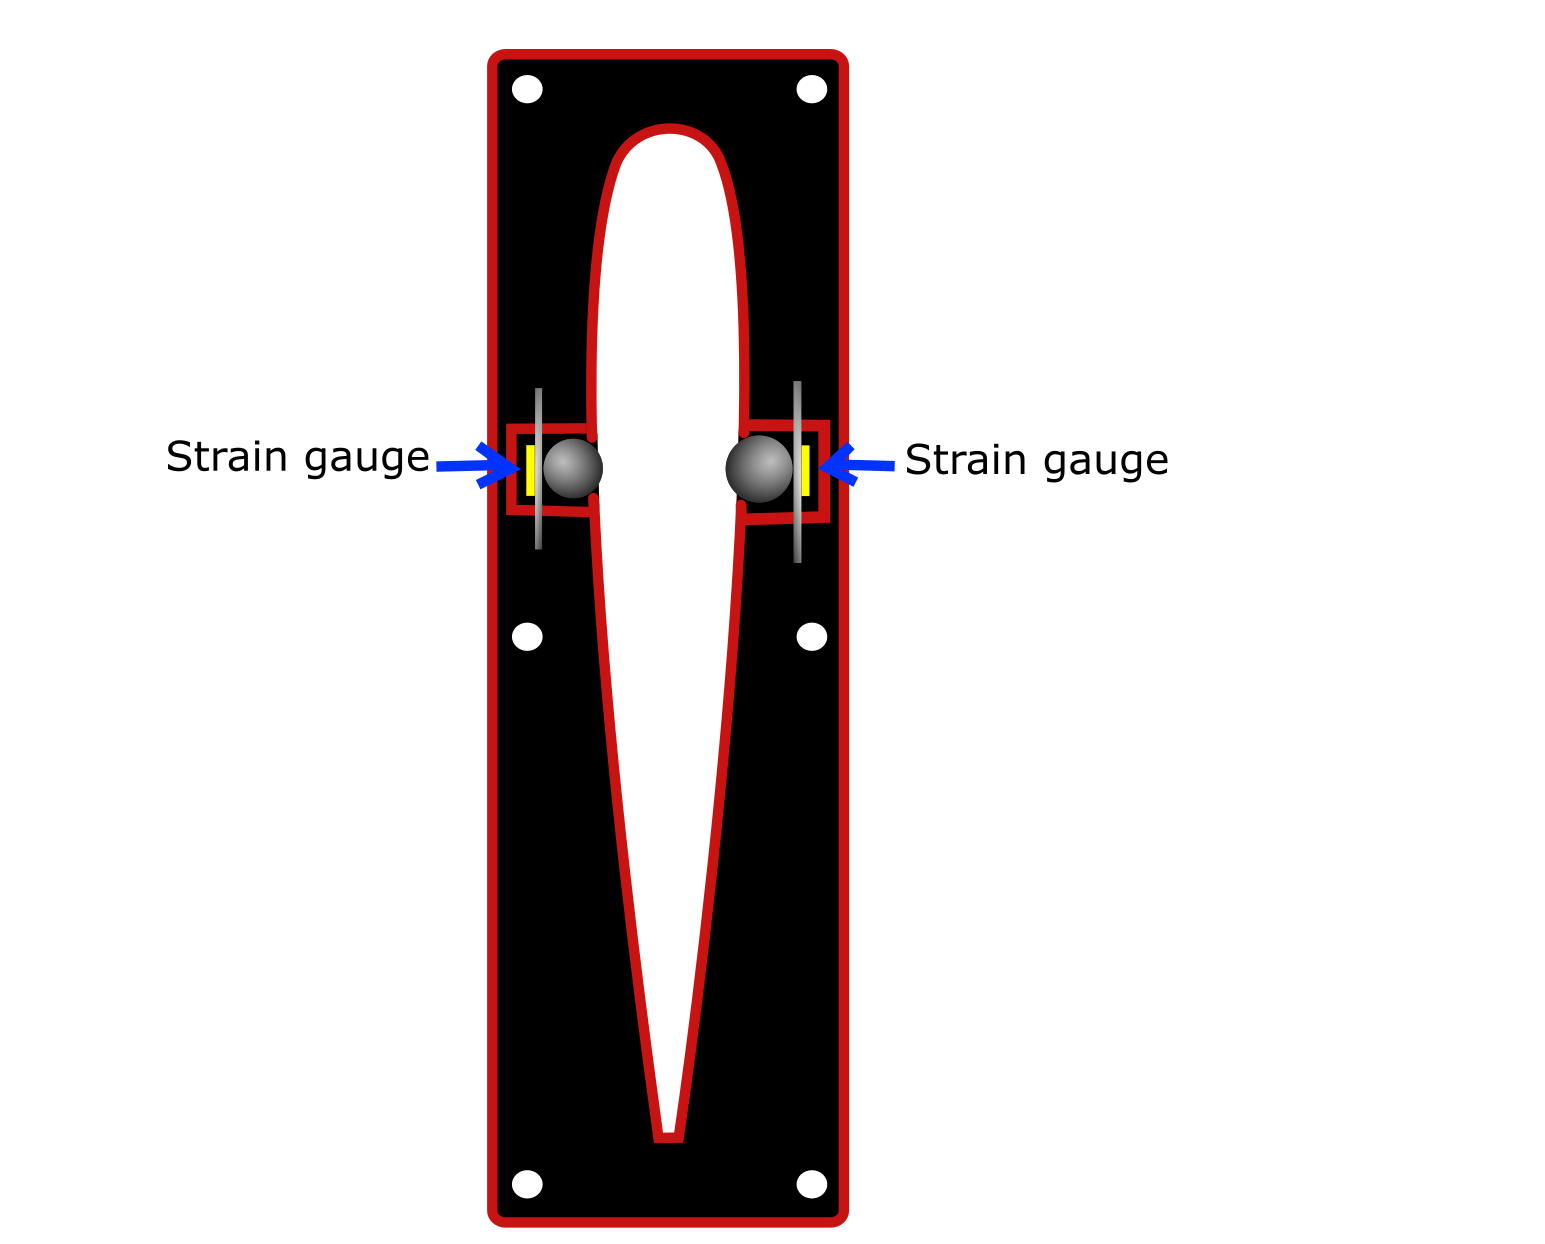
\includegraphics[width = 10cm]{Figures/Prototyp_1.png}
	\caption{Function of first prototype.}
	\label{Press_sens_impl}
\end{center}
\end{figure}



\subsubsection{The prototype}
To integrate the gauges, a prototype was designed to show how the measurements would be made. The prototype shown in \autoref{Press_sens_prot_1} is a bit bigger than the intended solution for this project but it is good to see how it would be constructed. The board goes on the outside and can easily slide up and down past the steel bead. The bead itself is kept inside a small space where it can move in and out.

The prototype of the pressure sensor was created in order to show the function of this sensor and to help the thought process involved in the improving of this design.

\begin{figure}[H]
\begin{center}
	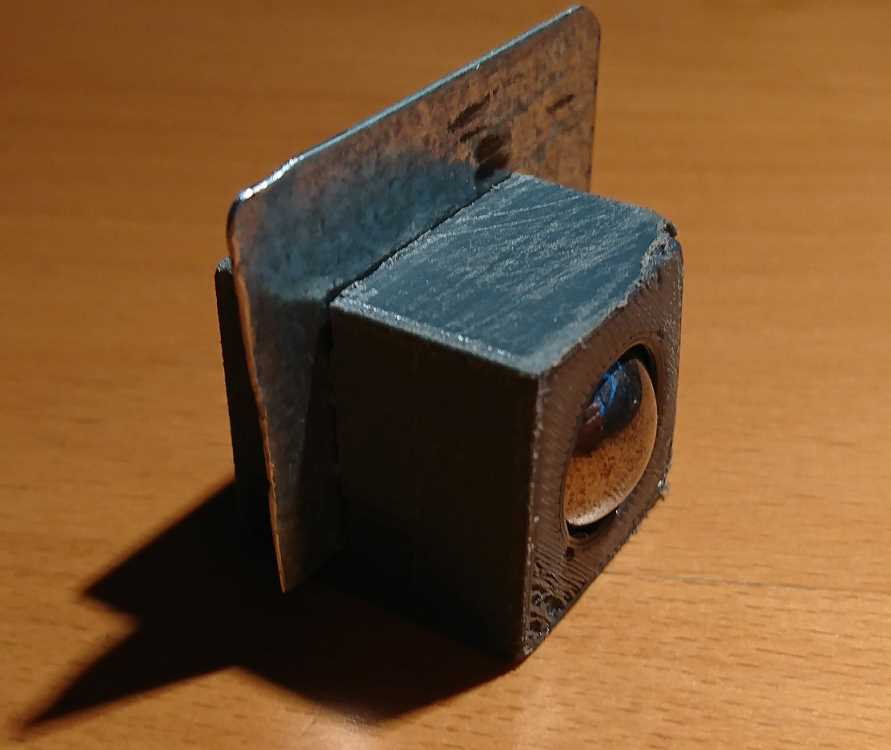
\includegraphics[width = 10cm]{Figures/Press_sens_prot_1.jpg}
	\caption{First prototype of a force sensor.}
	\label{Press_sens_prot_1}
\end{center}
\end{figure}

The force is measured at the back on the plate. The deflection of this plate will be used to measure the strain with strain gauges. 
The gauge itself will measure a small difference in resistance. This small difference is going to be difficult to measure without any amplifying circuit connected. With a such small signal the system might have issues with noise. Another problem is the signal might drift, and therefore make different measurements as the circuit is running. And finally, with the measured values getting amplified with a big amount the resulting signal may be off by a large amount. 

In the second prototype load cells, which are sensors that utilizes strain gauges to measure forces where chosen for this purpose. The difference in this prototype is instead of having a metal plate, it can be built with a piece of plastic or rubber which can deform so the force is distributed directly to the sensor. By implementing load cells, a lot of time was saved in troubleshooting. And by having a sensor unit, the modified mounting plate will be easier to produce. A illustration of this setup can be seen in \autoref{Press_sens_prot_2}
 
\begin{figure}[H]
\begin{center}
	
\includegraphics[width = 10cm]{Figures/Press_sens_func_2.png}
	\caption{Function of second prototype.}
	\label{Press_sens_prot_2}
\end{center}
\end{figure}



\subsubsection{Sensor}
The force from the board on the mounting plate will be considerable high. The actual force is something that is not known for sure. The initial assumption was that a load cell with a $90.75$ kg force range should be enough. If the sensor will be maxed out, the cell its rated for a $150\%$ overload without causing some damage to the sensor.  

The chosen sensor for this application is the compression load cell called FX1901\cite{load_cell}. 
From the datasheet, the voltage readings of this part could be calculated. The maximum voltage difference is calculated to be around $180mV$. See \autoref{Load_cell}
\begin{figure}[H]
\begin{center}
	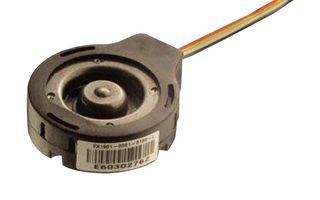
\includegraphics[width = 10cm]{Figures/Load_cell.png}
	\caption{Load cell, FX1901}
	\label{Load_cell}
\end{center}
\end{figure}


\subsection{Amplifier}
With such a small signal, an amplifier is needed to get good measurements. A good measurement signal to the \gls{mcu} should be between$0-3.3$ volts. Since the maximum value from the load cell is $180mV$ a signal of $3.3$ volts is achieved by an amplification gain of around $20$.  
A suitable amplifier needs to be chosen from this implementation. Inspiration is taken from The University of Chicago\cite{UoC} in an experiment where they use this exact load cell together with an instrumental amplifier called INA125. This amplifier more advanced and has more features than other amplifiers.  

In the same family of instrument amplifiers, the model called INA126\cite{ina_126} was selected as a less complicated and more power efficient solution.  
This amplifier has a smaller power draw due to simpler functionality and less precision. But for this application it is sufficient.  
The implementation is easy and the gain can easily be determined by connection a resistor Rg between two pins on the amplifier. See  \autoref{INA126}

\begin{figure}[H]
\begin{center}
	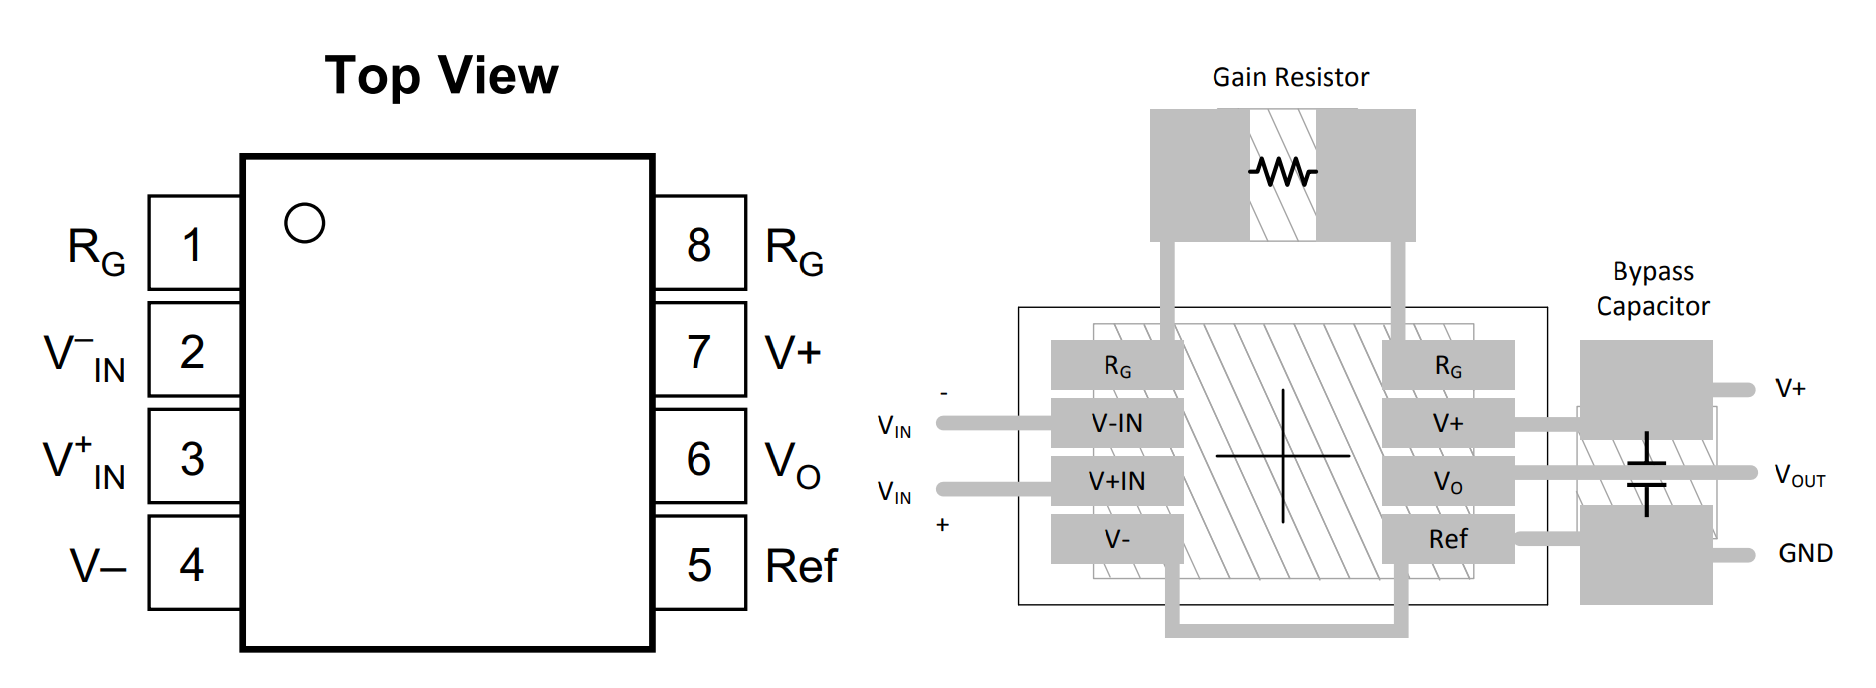
\includegraphics[width = 10cm]{Figures/INA126_pinout.png}
	\caption{Amplifier for the load cell signal.}
	\label{INA126}
\end{center}
\end{figure}

The gain is calculated with the following equation.  

\begin{equation}
\textrm{Gain} = 5 + \frac{80~\textrm{k}\Omega}{R_G}
\end{equation}

In order to adjust the gain of the amplifier the resistor $R_G$ is set to a fixed resistor in series with a potentiometer.


\subsection{Height of centerboard sensor}
The height of the daggerboard is a crucial measurement in dinghy sailing. The daggerboard not only gives the dinghy a corresponding force to the sail, the board can also be a danger if you sail in running wind. One of the best implementations of a height sensor would be the use of a linear wire distance sensor. This sensor measures how far a wire is pulled, which gives a very accurate measurement. This solution can be totally watertight and concealed in the main centerplate. Another solutions is to use some type of light sensor. 

\subsubsection{Sensors}


A suitable product was found, it is accurate and reliable, the Micro epsilon mk30\cite{micro-epsilon-mk30}.

It's physical volume in small enough with a size of 3x5cm. As the product have tight space constraints this would probably fit inside the case. As the sensors price was about 2000kr, it was deemed to expensive. If no other solution would work as intended this might have been considered again.

\begin{figure}[H]
\begin{center}
	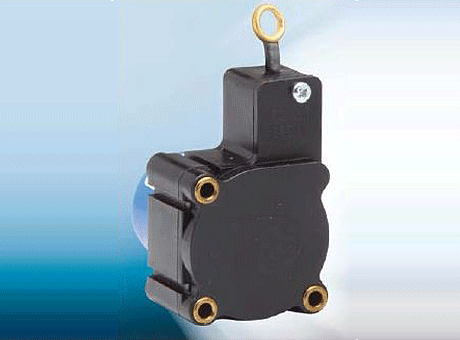
\includegraphics[width = 10cm]{Figures/microepsilon_mk30.png}
	\caption{Linear draw wire sensor, Micro epsilon MK30.}
	\label{Draw_sensor}
\end{center}
\end{figure}



Light sensors have also been considered. This would be implemented with the use of a plate placed on top of the dagger-board and with the light being sent up to this panel, the height can be calculated. First, we looked into some \gls{ir}-sensors. They will send the signal in a widespread which will make the distance measurement troublesome as this signal has just a small plate to bounce off.

With the use of a \gls{lidar} system, we can point our light signal at an exact spot and then get an exact measurement of the height.  
Many of the \gls{lidar} systems found was both too large and expensive to be implemented in this project.
But a product called "micro-lidar" could be used, as it has a small form factor, is easy to implement and is not to expensive.
The chosen module is the VL53L0X from Adafruit\cite{micro_lidar}. 

\begin{figure}[H]
	\centering
	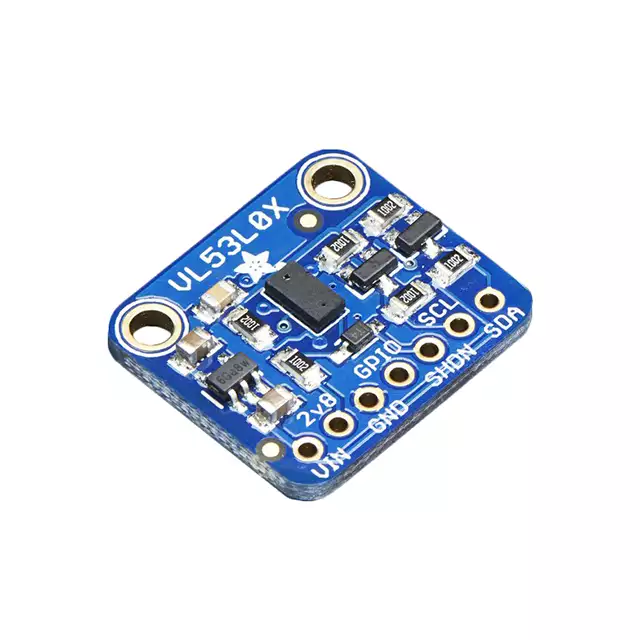
\includegraphics[width = 10cm]{Figures/Adafruit_height_sensor.png}
	\caption{Time of flight, $\mu$\gls{lidar}, distance sensor Adafruit VL53L0X.}
	\label{micro_lidar}
\end{figure}

It can measure heights up to one meter with great accuracy and communicates with \gls{i2c}.

By the fact that the sensor must be waterproof the signal has to go through a medium. The medium can be some type of transparent plastic or glass.   

All the information about this sensor and the usage of a cover widow can be found in the specific datasheet: “VL53L0X ranging module cover window guidelines” \cite{Tof_cover}. The maximum thickness of the cover window together with the air gap between the sensor and the window is 2 mm. That is the parameters that need to be considered. To reflect the signal a detection plate is constructed and fastened to the top of the daggerboard. This plate is level with the sensor and has a white underside for best performance of the sensor. In the case the sensor is mounted behind a thin epoxy window witch was to thick at the beginning but was sanded down to a sutible thickness. The final window were then polished to a crystal clear finish for the best measurements. 

\begin{figure}[H]
	\centering
	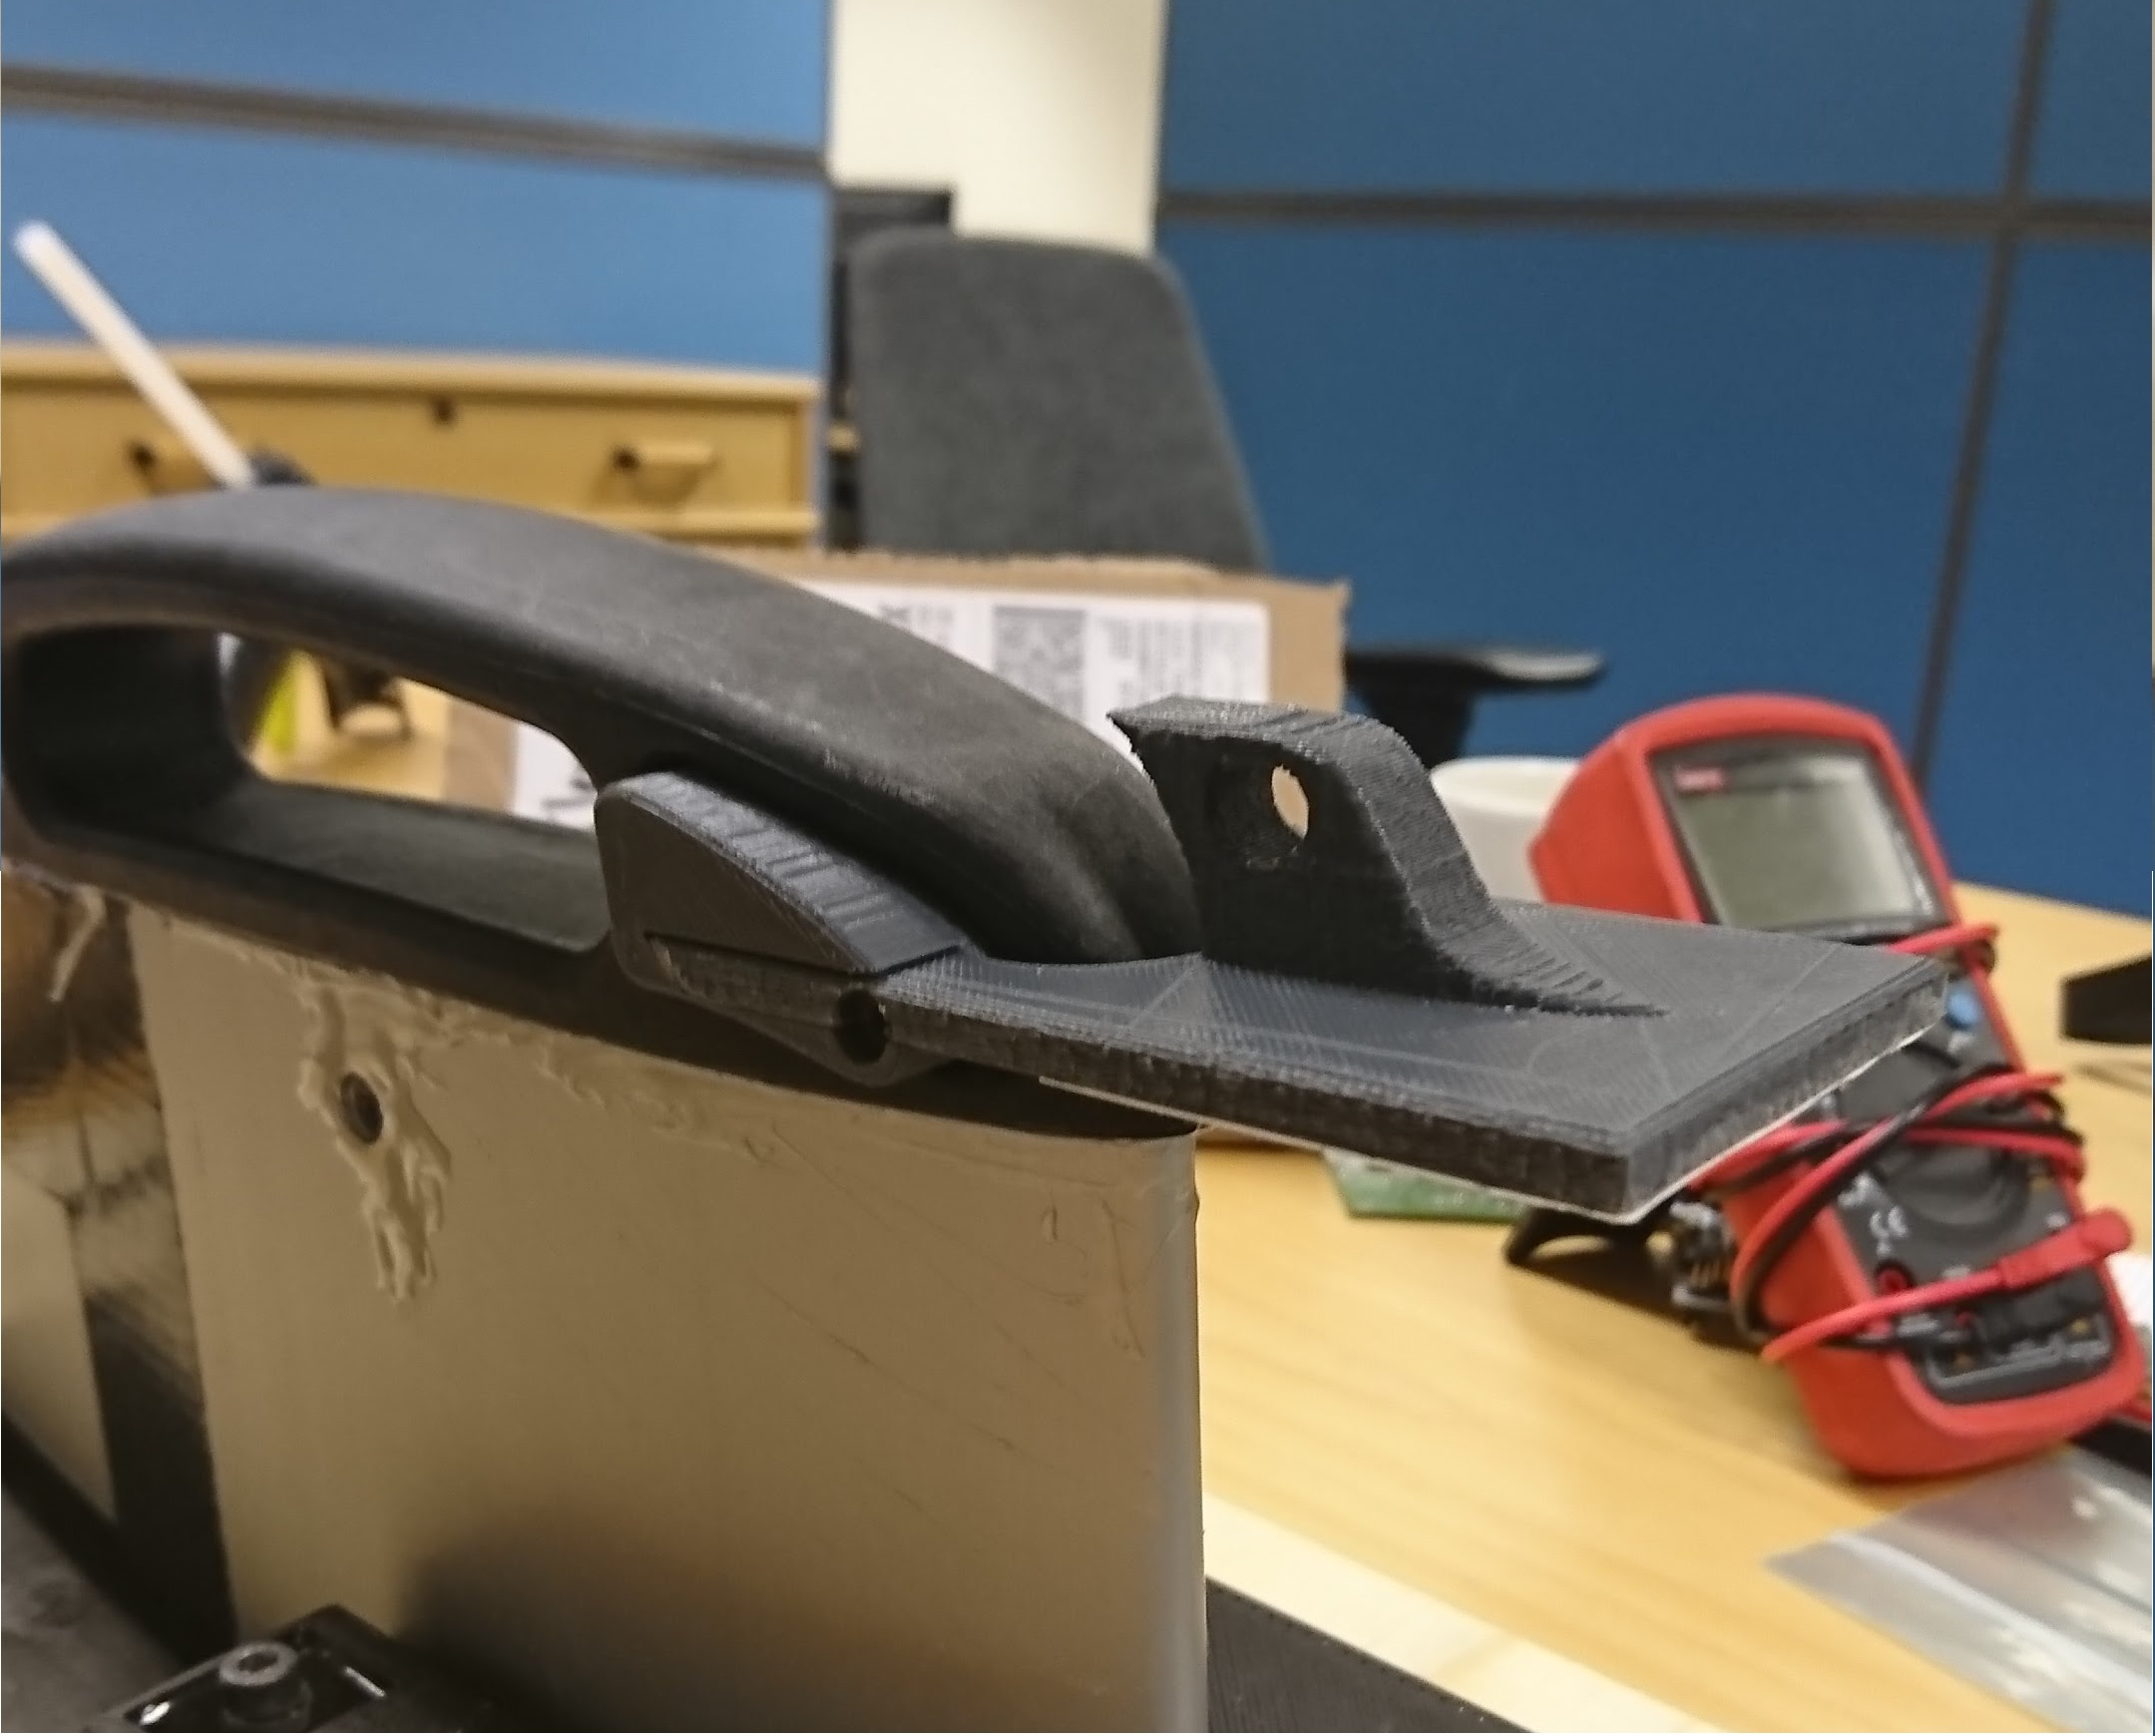
\includegraphics[width = 10cm]{Figures/height_measure.jpg}
	\caption{Height measurement model.}
	\label{height_measure}
\end{figure}


\subsubsection{Results}

The sensor works very well in the open air and can detect heights up to 1.5 meters with great accuracy. It also works well when used behind a thin transparent plastic cover. With a 1mm thin transparent plastic cover the maximum heigt measurement is decresed to about one meter. 

The measurement is heavily dependent on the the finish of the window, if there is small imperfections on the window such as scratch the sensor can't take measurements.

As there will always be water around and on the center plate the light that is sent might get scattered out off sight, even a small water droplet in between the sensor and the panel might cause a fault in the measurement.  

This system can definitively be improved in the future with either a completely different measurement system or with a better implementation of the window cover. The window cover probably would work better if the cover was molded in a convex form, which could lead off the water droplets formed on the window surface. This in cooperation with a surface finish that repels water, such as a hydrophobic coating would be a great solution. 
